%
%
%

\documentclass{BIThesis-Master}

\begin{document}

% ==================== %
% ===== 前置部分 ===== %
% ==================== %

%%%%% 封面 %%%%%
\makeCover

%%%%% 题名页 %%%%%
% 中文题名页
\classification{TQ028.1}
\UDC{540}
\title{形状记忆聚氨酯的合成及其在纺织中的应用}
\author{***}
\school{材料学院}
\mentor{***教授}
\chairman{***教授}
\degree{工学硕士}
\major{材料科学与工程}
\institute{北京理工大学}
\defenseDate{2009年6月}
\makeTitlePage
% 英文题名页
\titleEN{Synthesis and Application on textile of the Shape Memory Polyurethane}
\authorEN{***}
\schoolEN{Material Science and Engineering}
\mentorEN{Prof. ***}
\chairmanEN{Prof. ***}
\degreeEN{Master of Philosophy}
\majorEN{Material Science and Engineering}
\instituteEN{Beijing Institute of Technology}
\defenseDateEN{June, 2009}
\makeTitlePageEN

%%%%% 竖排页 %%%%%
\makeVerticalTitlePage

%%%%% 版权使用授权及研究成果声明 %%%%%
\makeOriginalityPage

%%%%% 摘要(中、英文) %%%%%
%
%
%

\begin{abstract}
  本文……。({\color{blue}{摘要是一篇具有独立性和完整性的短文,应概括而扼要地反映出本论文的主要内容。包括研究目的、研究方法、研究结果和结论等,特别要突出研究结果和结论。中文摘要力求语言精炼准确,硕士学位论文摘要建议500~800字,博士学位论文建议1000~1200字。摘要中不可出现参考文献、图、表、化学结构式、非公知公用的符号和术语。英文摘要与中文摘要的内容应一致。}})

  \keywords{形状记忆;聚氨酯;织物;合成;应用 ({\color{blue}{一般选3~8个单词或专业术语,且中英文关键词必须对应。})}}
\end{abstract}

\begin{abstractEN}
  In order to exploit ……

  \keywordsEN{shape memory properties; polyurethane;textile;synthesis;application}
\end{abstractEN}


%%%%% 目录 %%%%%
\TOC

% ==================== %
% ===== 主体部分 ===== %
% ==================== %

%%%%% 正文 %%%%%
%
%
%

\chapter{绪论}
\label{chap:intro}

\section{本论文研究的目的和意义}

近年来,随着人们生活水平的不断提高,人们越来越注重周围环境对身体健康的影响。作为服装是人们时时刻刻最贴近的环境,尤其是内衣,对人体健康有很大的影响。由于合时刻刻最贴近的环境,尤其是内衣,对人体健康有很大的影响。由于合成纤维的衣着舒适性、手感性,天然纤维的发展又成为人们关注的一大热点。

……

\section{国内外研究现状及发展趋势}

\subsection{形状记忆聚氨酯的形状记忆机理}

形状记忆聚合物(SMP)是继形状记忆合金后在80年代发展起来的一种新型形状记忆材料。形状记忆高分子材料在常温范围内具有塑料的性质,即刚性、形状稳定恢复性;同时在一定温度下(所谓记忆温度下)具有橡胶的特性,主要表现为材料的可变形性和形变恢复性。即“记忆初始态-固定变形-恢复起始态”的循环。

固定相只有物理交联结构的聚氨酯称为热塑性SMPU,而有化学交联结构称为热固性SMPU。热塑性和热固性形状记忆聚氨酯的形状记忆原理示意图如图\ref{fig:diagram}所示。

\begin{figure}
  \centering
  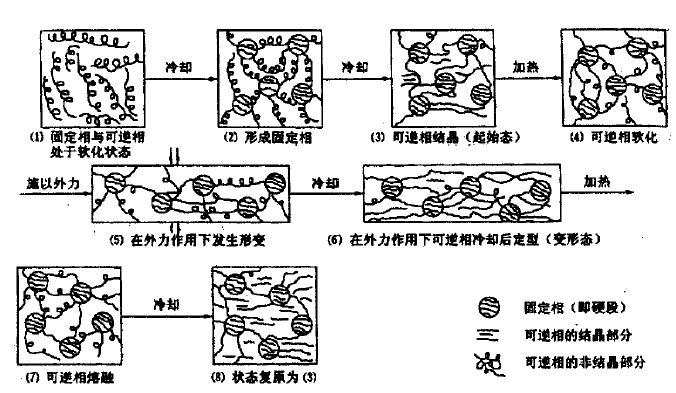
\includegraphics[width=0.75\textwidth]{assets/figure1.png}
  \caption{热塑性形状记忆聚氨酯的形状记忆机理示意图}
  \label{fig:diagram}
\end{figure}

\subsection{形状记忆聚氨酯的研究进展}

首例SMPU是日本Mitsubishi公司开发成功的……。

\subsection{水系聚氨酯及聚氨酯整理剂}

水系聚氨酯的形态对其流动性,成膜性及加工织物的性能有重要影响,一般分为三种类型\cite{Jiang2005Size} ,如表\ref{tab:category}所示。

\begin{table}
  \centering
  \caption{水系聚氨酯分类}
  \label{tab:category}
  \begin{tabular*}{0.9\textwidth}{@{\extracolsep{\fill}}cccc}
    \toprule
      类别			&水溶型		&胶体分散型		&乳液型 \\
    \midrule
      状态			&溶解$\sim$胶束	&分散		&白浊 \\
      外观			&水溶型		&胶体分散型		&乳液型 \\
      粒径$/\mu m$	&$<0.001$		&$0.001-0.1$		&$>0.1$ \\
      重均分子量	&$1000\sim 10000$	&数千$\sim 20万$ &$>5000$ \\
    \bottomrule
  \end{tabular*}
\end{table}

由于它们对纤维织物的浸透性和亲和性不同,因此在纺织品染整加工中的用途也有差别,其中以水溶型和乳液型产品较为常用。另外,水系聚氨酯又有反应性和非反应性之分。虽然它们的共同特点是分子结构中不含异氰酸酯基,但前者是用封闭剂将异氰酸酯基暂时封闭,在纺织品整理时复出。相互交联反应形成三维网状结构而固着在织物表面。

……


%%==================================================
%% modified based on BIT-Thesis-template v1.5
%% author: Zheng Shuai <i AT iamzs.win>
%%==================================================

\begin{conclusion}

  本文采用……。{\color{blue}(结论作为学位论文正文的最后部分单独排写,但不加章号。结论是对整个论文主要结果的总结。在结论中应明确指出本研究的创新点,对其应用前景和社会、经济价值等加以预测和评价,并指出今后进一步在本研究方向进行研究工作的展望与设想。结论部分的撰写应简明扼要,突出创新性。)}

\end{conclusion}


%%%%% 参考文献 %%%%%
\bibliography{mainmatter/reference}

% ==================== %
% ===== 后置部分 ===== %
% ==================== %

%%%%% 附录(必要时) %%%%%
\appendix
\renewcommand\theequation{\Alph{chapter}--\arabic{equation}}
\renewcommand\thefigure{\Alph{chapter}--\arabic{figure}}
\renewcommand\thetable{\Alph{chapter}--\arabic{table}}

%
%
%

\chapter{附录}

附录相关内容…


%%%%% 攻读学位期间发表论文与研究成果清单 %%%%%
%
%
%

\begin{publications}{99}
  \item\textsc{高凌}. {交联型与线形水性聚氨酯的形状记忆性能比较}[J].化工进展, 2006, 532-535.(核心期刊)
\end{publications}


%%%%% 致谢 %%%%%
%%==================================================
%% modified based on BIT-Thesis-template v1.5
%% author: Zheng Shuai <i AT iamzs.win>
%%==================================================

\begin{thanks}

  本论文的工作是在导师……。

\end{thanks}


%%%%% 作者简介 %%%%%
%%==================================================
%% resume.tex  for BIT Master Thesis
%% modified by yang yating
%% version: 0.2
%% last update: Feb 16th, 2017
%%==================================================


\begin{resume}

\begin{resumesection}{基本情况}
xxx,男,上海人,1985 年~12 月出生,未婚,
上海交通大学物理系在读博士研究生。
\end{resumesection}

\begin{resumeli}{教育状况}
XXXX 年~9 月至~XXXX 年~7 月,上海交通大学, 本科,专业:XXXX

XXXX 年~9 月至~XXXX 年~7 月,上海交通大学, 硕士研究生,专业:XXXX

XXXX 年~9 月至~XXXX 年~7 月,上海交通大学,
博士研究生(提前攻读博士),专业:XXXX
\end{resumeli}

\begin{resumeli}{工作经历}
无。
\end{resumeli}

\begin{resumeli}{研究兴趣}
XXXXXXX。
\end{resumeli}

\begin{resumeli}{联系方式}
通讯地址:上海市闵行区东川路800号,上海交通大学物理系

邮编:200240

E-mail: abcde@sjtu.edu.cn
\end{resumeli}

\end{resume}


\end{document}
